\chapter{Introduzione}\label{ch:introduzione}
	
	L'``\textit{Istituto Ortopedico Gaetano Pini}''\cite{istituto} di Milano è un istituto, fondato nel 1874, specializzato nella cura e nella riabilitazione delle malattie ortopediche e reumatologiche, sede di didattica e ricerca universitaria.

	Nel documento, oltre al nome dell'Istituto, ci si riferisce a questo anche come ``\textit{\istituto}'' o  ``\textit{\proponente}''.
	
	``\textit{\azienda}''\cite{sito_azienda} è un'azienda che si occupa principalmente di fornire assistenza tecnica alle imprese che desiderano rimodenare il proprio sistema informatico.

	Nel documento, oltre al nome dell'azienda, ci si riferisce a questa anche come ``\textit{\offerente}''.

\section{Scopo del documento}\label{sec:scopo_documento}
	
	In questo documento viene dettagliata la fase di \textit{\rollout} del \textit{nuovo \helpdesk}, secondo quanto richiesto nel \textit{Capitolato Tecnico} fornito dall'\istituto.
	
	In tale capitolato viene descritto l'appalto per la progettazione, realizzazione, manutenzione, evoluzione e gestione del sistema informatico aziendale dell'Azienda Ospedaliera.
	
	Come richiesto nel capitolato, vengono inoltre descritte le attività di revisione delle logiche operative esistenti.
	
	\subsection{Organizzazione del documento}\label{sec:organizzazione_documento}
	
		Il documento è stato suddiviso nei seguenti capitoli:
		\begin{enumerate}[noitemsep]
			
			\item \hyperref[ch:introduzione]{Introduzione}: in questo primo capitolo viene descritto il contenuto del documento presentando concetti come la definizione della fase di \rollout, la durata del contratto, punti di contatto tra \azienda~e \istituto;
			
			\item \hyperref[ch:servizio_helpdesk]{Il servizio di \helpdesk}: in questo capitolo viene introdotto il servizio di \helpdesk, vengono elencati gli obiettivi del nuovo sistema secondo le richieste dell'\istituto~e viene spiegato come \azienda~propone che queste vengano compiute;
			
			\item \hyperref[ch:implementazione]{\textit{Deployment} del nuovo sistema informatico}: in questo capitolo vengono spiegate in dettaglio le fasi dell'implementazione del nuovo sistema informatico;
			
			\item \hyperref[ch:supporto]{Attività e risorse di supporto}: in questo capitolo vengono descritte le attività e le risorse di supporto necessarie al processo di \rollout;
			
			% \item \hyperref[ch:conclusioni]{Conclusioni}: in questo ultimo capitolo vengono fatte alcune considerazioni finali da parte di \azienda~riguardanti il progetto e l'appalto;
			
			% \item \hyperref[ch:appendice_a]{Appendice A}:
			
		\end{enumerate}
	
\section{Fase di \rollout}

	All'interno delle \textit{best practice} descritte nel framework \textit{ITIL V3}\cite{itil_website}, la fase di \rollout~fa parte del processo di \textit{Release and Deployment Management}, inserita nell'area di Service Transition.
	
	Tale processo ha lo scopo di pianificare e controllare il movimento delle release negli ambienti \textit{live} (o di \textit{produzione}) e di \textit{test}, assicurando che l'integrità dell'ambiente di produzione venga mantenuta e che le componenti siano rilasciate correttamente.
	
	A sua volta, tale processo viene suddiviso nei seguenti sottoprocessi:
	
	\begin{itemize}[noitemsep]
		\item \textit{Release Management Support}: fornisce linee guida e supporto per lo sviluppo delle release;
		\item \textit{Release Planning}: assegna le change, dopo essere state autorizzate, ai release packages e definisce la portata e i contenuti delle release. Inoltre, sviluppa uno schedule per build, test e deployment della release;
		\item \textit{Release Build}: emette tutti gli ordini di lavoro e le richieste di acquisto per lo sviluppo interno o l'acquisizione delle componenti della release, in modo da renderli disponibili per la fase di test;
		\item \textit{Release Deployment}: effettua il deploy delle componenti della release nell'ambiente di produzione. Inoltre, forma gli utenti e il personale operativo e si occupa di rilasciare informazioni e documentazione sulle release di cui è stato fatto il deploy;
		\item \textit{Early Life Support}: risolve problemi operativi nel periodo immediatamente successivo al rilascio, in cui è più probabile che essi si manifestino. Durante l’Early Life Support il \textit{Service Transition} affianca il \textit{Service Operations};
		\item \textit{Release Closure}: si occupa della chiusura formale di una release dopo essersi assicurati che i log e il database siano stati aggiornati.
	\end{itemize}

	\begin{figure}[h!]
		\centering
		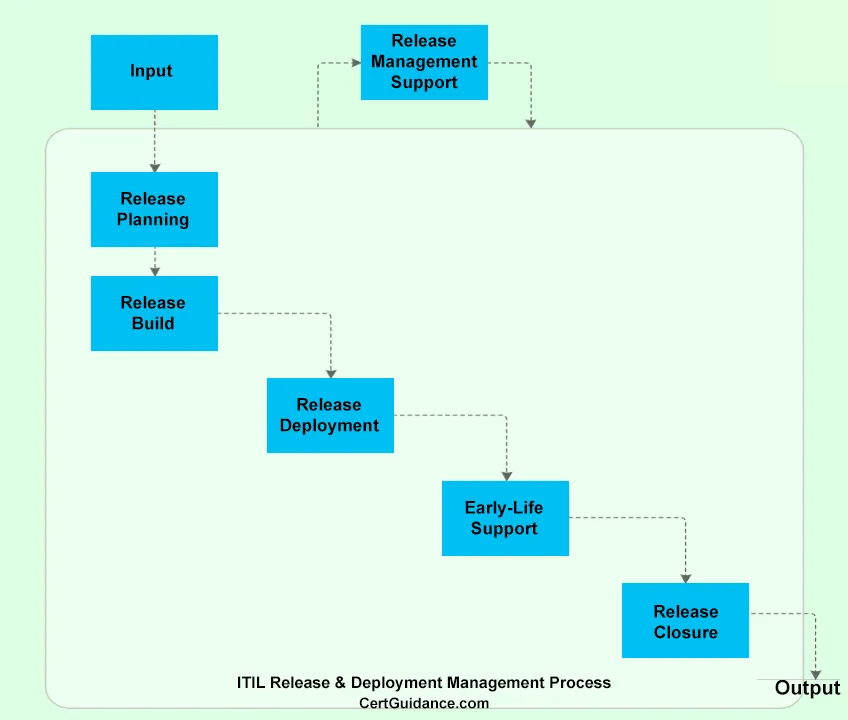
\includegraphics[width=\linewidth]{img/intro_rollout.png}
		\caption{Sottoprocessi di \textit{Release and Deployment Management}\cite{release_deployment_management}}
		\label{fig:intro_rollout}
	\end{figure}

%\section{Utenti e struttura aziendale}\label{sec:struttura_aziendale}
%	
%	Come descritto nel capitolato d'appalto fornito dall'Istituto, il nuovo sistema informatico è rivolto a tutti i dipendenti e ai clienti dei servizi che vengono offerti dalla struttura ospedaliera.
%	
%	Una descrizione più dettagliata degli utenti del servizio e della struttura vengono viene svolta nelle sezioni \ref{ch:servizio_helpdesk} e \ref{sec:utenti}.
	
	
\section{Durata del contratto}
	
	Nonostante la durata totale del contratto sia di nove anni, come descritto nella sezione 5.2 del capitolato fornito dal \proponente, la durata dell'implementazione da parte di \azienda~deve rientrare nei primi trenta mesi dalla firma del contratto.
	
	Siccome potrebbero avvenire cambiamenti \textit{in corso d'opera} dal momento della firma del contratto, questo documento verrà costantemente aggiornato in maniera da rispecchiare correttamente la pianificazione corrente della fase di \rollout.

%\section{Costo per la fornitura del servizio}
%	\hl{Ha senso scrivere questa sezione? Con che tipo di dati posso riempirla? Che stima faccio?}
	
\section{Penali}

	\azienda~si impegna a rispettare la pianificazione fissata per l'implementazione, delineata in \ref{sec:pianificazione}, prendendosi carico delle penali che possono essere imposte in caso di ritardi, o altri eventuali errori, come descritto nel ``\textit{Capitolo 5: Requisiti per i Servizi}'' del capitolato d'appalto fornito dal \proponente.
	
\section{Punti di contatto dell'azienda}

	\azienda~si impegna a fornire completa disponibilità dei propri contatti con l'\istituto~per qualsiasi comunicazione riguardante il presente documento e il servizio descritto.

	Nella seguente tabella vengono indicati i principali punti di contatto tra \azienda~e l'\istituto.
	\begin{table}[H]
		\renewcommand\arraystretch{2}
		\centering
		\begin{tabular}{|>{\raggedright\arraybackslash}m{3.25cm}|m{4.25cm}|m{4cm}|}
			\hline
			\rowcolor{pantone}
			\multicolumn{1}{|>{\centering\arraybackslash}m{3.25cm}|}{\color{white}\textbf{Ruolo}} &
			\multicolumn{1}{>{\centering\arraybackslash}m{4.25cm}|}{\color{white}\textbf{Nome}} &
			\multicolumn{1}{>{\centering\arraybackslash}m{4cm}|}{\color{white}\textbf{Indirizzo e-mail}}\\
			\hline
			Responsabile privacy			& 	MARIA AMERIO 		& M.AMERIO@\mailazienda		\\\hline
			Responsabile qualità			& 	ANDREA TORCHIO 		& A.TORCHIO@\mailazienda	\\\hline
			Amministratore database			& 	GIOVANNI GAMBA 		& G.GAMBA@\mailazienda		\\\hline
			Responsabile analisi			& 	ROBERTO BARBERO 	& R.BARBERO@\mailazienda	\\\hline
			Responsabile progettazione		& 	ANTONIO PENNA 		& A.PENNA@\mailazienda		\\\hline
			
		\end{tabular}
		\renewcommand\arraystretch{1}
		\caption{Tabella con gli indirizzi e-mail e i ruoli di riferimento}
	\end{table}	
	